\documentclass[11pt]{article}
\usepackage[T1]{fontenc}
\usepackage{lmodern}
\usepackage[margin=1in]{geometry}
\usepackage{amsmath,amssymb,amsthm,mathtools}
\usepackage{microtype}
\usepackage{tikz}
\usepackage{listings}
\lstset{basicstyle=\ttfamily\footnotesize,columns=fullflexible,keepspaces=true,
  literate={∀}{{$\forall$}}1 {∈}{{$\in$}}1 {∉}{{$\notin$}}1
  {→}{{$\to$}}1 {ℝ}{{$\R$}}1 {θ}{{$\theta$}}1
  {∨}{{$\lor$}}1 {≤}{{$\leq$}}1}
\usepackage[colorlinks=true,linkcolor=blue,citecolor=blue,urlcolor=blue]{hyperref}
\hypersetup{pdftitle={Strongly cospectral sets in seven-dimensional cubelike graphs},pdfauthor={P. Graham}}
\newtheorem{theorem}{Theorem}[section]
\newtheorem{lemma}[theorem]{Lemma}
\newtheorem{proposition}[theorem]{Proposition}
\newtheorem{corollary}[theorem]{Corollary}
\theoremstyle{definition}
\newtheorem{definition}[theorem]{Definition}
\newcommand{\F}{\mathbb F}
\newcommand{\R}{\mathbb R}
\newcommand{\Z}{\mathbb Z}
\newcommand{\Cay}{\operatorname{Cay}}
\newcommand{\supp}{\operatorname{supp}}
\title{Strongly cospectral sets in seven-dimensional cubelike graphs}
\author{P. Graham\\ \small\url{https://orcid.org/0009-0007-8493-1505}}
\date{October 23, 2026}
\begin{document}
\maketitle
\begin{abstract}
Two vertices of a graph are strongly cospectral if their orthogonal
projections onto each adjacency eigenspace agree up to sign.
\'Arnad\'ottir and Godsil asked in 2021 whether their upper bound
$2^{\lceil d/2\rceil-1}$ for the size of a pairwise strongly cospectral
set in a cubelike graph on $2^d$ vertices, $d\geq3$, is tight in every
dimension in its range.
We prove that every such set in every cubelike graph on $128$ vertices
has size at most four, whereas their bound gives eight.
Their connected construction attains four, so the maximum in dimension
seven is exactly four and the all-dimensions tightness question has a
negative answer.
The proof combines character sums, congruences and a second-moment bound
with an exact finite inequality certified by linear programming duality.
The universal upper bound, including the certificate checks, is formalized
in Lean; attainment is checked separately.
\end{abstract}

\noindent Computer-assisted; not yet reviewed by experts.

\smallskip
\noindent The proofs, the Lean formalization, the certificate checkers and the text
were produced by AI models (from OpenAI and Anthropic), working under the
author's direction.

\section{Introduction}
A \emph{cubelike graph} is a Cayley graph $\Cay(\F_2^d,S)$, where
$S\subseteq\F_2^d\setminus\{0\}$: vertices $x$ and $y$ are adjacent when
$x+y\in S$. For its adjacency matrix $A$, let $E_\theta$ be the orthogonal
projection onto the eigenspace with eigenvalue $\theta$, and let $e_x$ be
the coordinate vector at $x$. Vertices $x,y$ are \emph{strongly cospectral}
when $E_\theta e_x=\pm E_\theta e_y$ for every eigenvalue $\theta$, with
the sign allowed to depend on $\theta$.

\begin{theorem}\label{thm:main}
Let $S\subseteq\F_2^7\setminus\{0\}$. Every set of pairwise strongly
cospectral vertices in $\Cay(\F_2^7,S)$ has at most four elements.
This bound is attained by a connected graph.
\end{theorem}

No connectivity or degree assumption is imposed on the upper bound; in
particular, it includes the empty connection set.

\'Arnad\'ottir and Godsil~\cite{AG}, Corollary~8.3, proved that a pairwise
strongly cospectral set in a cubelike graph on $2^d$ vertices has size at
most $2^{\lceil d/2\rceil-1}$ for $d\geq3$.
Their Example~8.4 attains this bound for $d=3,4,5,6$.
In Section~11 they asked:
\begin{quote}
``Is the upper bound on the size of strongly cospectral sets in cubelike
graphs tight in all dimensions?''
\end{quote}
The question appeared in their first preprint, posted September 15, 2021;
the journal article appeared in 2023.
At $d=7$ their bound is eight. Theorem~\ref{thm:main} reduces it to four,
and hence answers their question negatively.

The contribution here is the upper bound four in dimension seven.
The character criterion used below is the specialization of
\'Arnad\'ottir--Godsil's Theorem~10.1 to an elementary abelian $2$-group,
building on the normal-Cayley character criterion of Peter Sin and
Julien Sorci~\cite[Theorems~2.3 and~2.4]{SinSorci}, as credited in
\'Arnad\'ottir--Godsil's Theorem~5.2.
The attaining connected example is \'Arnad\'ottir--Godsil's Theorem~10.2.
Their bound follows from eigenvalue multiplicities and a global
second-moment argument. Here the hardest step is a stronger finite
inequality, certified by linear programming duality. It combines
disjointness of the eigenvalue values on eight character cosets with
their individual means, their residues modulo four, and Parseval's
identity. The earlier multiplicity bound does not impose these
coset restrictions together.

This result does not bound the size of strongly cospectral sets uniformly
over all dimensions. Peter Sin~\cite{Sin}, in work first posted in 2022,
constructed cubelike graphs with arbitrarily large strongly cospectral
classes. The maximum in dimensions eight and higher is not determined
here. The computational examples and Sage code of \'Arnad\'ottir and
Godsil, and Gordon Royle's cubelike graph lists credited by them,
are prior work.

Section~\ref{sec:overview} explains the proof. Sections~\ref{sec:characters}
and~\ref{sec:moments} derive the character and moment restrictions.
Section~\ref{sec:finite} reduces the upper bound to a finite inequality,
and Section~\ref{sec:certificates} gives the exact certificate argument.
Section~\ref{sec:example} describes the known
attaining graph. The final section states the scope of the computation
and formalization.

\section{Proof overview}\label{sec:overview}
The proof rules out a strongly cospectral class of size eight.
Write $V=\F_2^7$. For a character indexed by $a\in V$, the corresponding
adjacency eigenvalue is
\[
 \lambda_a=\sum_{s\in S}(-1)^{a\cdot s},
\]
where the dot product takes values in $\F_2$.
The vertices strongly cospectral with zero form a subspace $K(S)$ of $V$:
a vector $g$ lies in it precisely when $a\cdot g$ is constant on each
\emph{eigenvalue fiber}, meaning a set $\{a\in V:\lambda_a=\theta\}$.
The sum $\sigma=\sum_{s\in S}s$ also belongs to $K(S)$.
Consequently, if $|K(S)|\geq8$, a change of basis places a
three-dimensional subspace $H$ inside $K(S)$ with $\sigma\in H$.

The eight cosets of $H^\perp$ then have disjoint sets of eigenvalue
values. All values in a given coset have a prescribed residue modulo
four. Their full coset means depend only on $B=S\cap H$, which has at
most seven elements. After removing the trivial character from the
zero coset, its remaining mean also depends on $n=|S|$.
The sum of all squared eigenvalues is fixed by Parseval's
identity: it is $128|S|$.

For each coset, retain only the nearest eigenvalue values on either side
of its mean. These two endpoints give a lower bound for that coset's
sum of squares. They must satisfy the residue restriction and must avoid
the endpoints chosen by every other coset. The eigenvalue $|S|$ at the
trivial character is treated separately. This leaves a finite question
about eight pairs of integers, parameterized by $|S|$, $B$, and $\sigma$.

The hard finite inequality is that every permitted selection of these
pairs has total lower bound strictly greater than $128|S|$.
It is certified by assigning nonnegative penalties to endpoint values.
The penalty-adjusted minimum for each coset can be computed independently;
subtracting the total available penalty gives a valid lower bound because
each endpoint value can be used by at most one coset.
Exact certificates make that lower bound exceed $128|S|$ in every case.
The resulting contradiction proves the upper bound.

\section{The character criterion and normalization}\label{sec:characters}
We identify strongly cospectral classes with a subspace defined by
character eigenvalues and put a hypothetical large class in a fixed position.
Throughout the proof, $V=\F_2^7$, $S\subseteq V\setminus\{0\}$, and
$n=|S|$. For $a\in V$, define
\begin{equation}\label{eq:lambda}
 \chi_a(x)=(-1)^{a\cdot x},\qquad
 \lambda_a=\sum_{s\in S}\chi_a(s),\qquad
 n_a=|\{s\in S:a\cdot s=1\}|.
\end{equation}
In particular, $\lambda_a=n-2n_a$. Define
\begin{equation}\label{eq:K}
 K(S)=\{g\in V:\lambda_a=\lambda_b\Longrightarrow
                  a\cdot g=b\cdot g\text{ for all }a,b\in V\}.
\end{equation}

\begin{lemma}[Character criterion]\label{lem:criterion}
For $x,y\in V$, the vertices $x$ and $y$ are strongly cospectral in
$\Cay(V,S)$ if and only if $x+y\in K(S)$.
The set $K(S)$ is a subspace, and its cosets are the strongly cospectral
classes.
\end{lemma}
\begin{proof}
The characters $\chi_a$ form an orthogonal basis of $\R^V$, with squared
norm $128$, and $A\chi_a=\lambda_a\chi_a$. Thus
\[
 E_\theta e_g=\frac1{128}
          \sum_{a:\lambda_a=\theta}\chi_a(g)\chi_a.
\]
By linear independence, this equals $\pm E_\theta e_0$ precisely when
$\chi_a(g)$ is constant over $a$ with $\lambda_a=\theta$.
This is exactly the condition $g\in K(S)$.
Translations are graph automorphisms, so the assertion for $x,y$ follows
by translating $x$ to zero. Finally, each condition defining $K(S)$ is
a homogeneous linear equation in $g$, and hence $K(S)$ is a subspace.
\end{proof}

\begin{lemma}\label{lem:sigma}
Put $\sigma=\sum_{s\in S}s$, where the sum is in $V$. Then
$\sigma\in K(S)$, and for every $a\in V$,
\begin{equation}\label{eq:residue}
 n_a\equiv a\cdot\sigma\pmod2,\qquad
 \lambda_a\equiv n-2(a\cdot\sigma)\pmod4.
\end{equation}
Here elements of $\F_2$ in integer congruences are represented by $0,1$.
\end{lemma}
\begin{proof}
The parity of $n_a$ is $\sum_{s\in S}a\cdot s=a\cdot\sigma$.
Equality of two eigenvalues implies equality of the corresponding
$n_a$, so it implies equality of the dot products with $\sigma$.
The second congruence follows from $\lambda_a=n-2n_a$.
\end{proof}

Let $e_1,\ldots,e_7$ denote the standard basis of $V$, and put
$H=\langle e_1,e_2,e_3\rangle$.
We encode a vector $\sum_i x_i e_i$ by the integer
$\sum_i 2^{i-1}x_i$. In particular, $H=\{0,\ldots,7\}$.
Addition of encoded vectors is bitwise exclusive-or, rather than
integer addition.

\begin{lemma}[Normalization]\label{lem:normal}
If $|K(S)|\geq8$, an invertible linear change of coordinates replaces
$S$ by a connection set for which $H\subseteq K(S)$ and $\sigma\in H$.
\end{lemma}
\begin{proof}
By Lemmas~\ref{lem:criterion} and~\ref{lem:sigma}, $K(S)$ is a subspace
of dimension at least three containing $\sigma$.
Choose a three-dimensional subspace of $K(S)$ containing $\sigma$;
this is possible also when $\sigma=0$.
Extend a basis of that subspace to a basis of $V$, and let $T$ map this
basis to the standard one. For the connection set $TS$,
\[
 \lambda^{TS}_a=\lambda^S_{T^{\mathsf T}a},\qquad
 K(TS)=T K(S),\qquad \sigma(TS)=T\sigma(S).
\]
The eigenvalue identity follows from $a\cdot Ts=(T^{\mathsf T}a)\cdot s$;
substitution in~\eqref{eq:K} gives the identity for $K$.
These identities give the required position.
\end{proof}

If a pairwise strongly cospectral set has more than four vertices,
Lemma~\ref{lem:criterion} gives $|K(S)|>4$.
The cardinality of a binary subspace is a power of two, so it is at least
eight. It therefore suffices to exclude the normalized situation of
Lemma~\ref{lem:normal}.

\section{Coset means, residues, and the second moment}\label{sec:moments}
We now derive the restrictions that cannot hold together in dimension
seven. Assume $H\subseteq K(S)$ and $\sigma\in H$.
Write $t=\sigma\in\{0,\ldots,7\}$, $B=S\cap H$, and $m=|B|$.
For $u\in\{0,\ldots,7\}$, define
\[
 C_u=\{a\in V:\text{the first three coordinates of }a\text{ equal }u\},
 \qquad \mu_u=\sum_{h\in B}(-1)^{u\cdot h}.
\]
The sets $C_u$ are the cosets of $H^\perp$; each has $16$ elements.
In this formula $u\cdot h$ is the three-coordinate binary dot product.

\begin{lemma}\label{lem:cosets}
The following hold:
\begin{enumerate}
\item If $u\ne w$, no eigenvalue value occurs both on $C_u$ and on $C_w$.
\item For $a\in C_u$, $-n\leq\lambda_a\leq n$ and
$\lambda_a\equiv n-2(u\cdot t)\pmod4$. Also $\lambda_0=n$.
\item The coset sums and total second moment are
\begin{equation}\label{eq:moments}
 \sum_{a\in C_u}\lambda_a=16\mu_u,\qquad
 \sum_{a\in V}\lambda_a^2=128n.
\end{equation}
In particular, $\mu_0=m$.
\end{enumerate}
\end{lemma}
\begin{proof}
If $u\ne w$, some $e_i\in H$, $1\leq i\leq3$, has different dot
products with $a\in C_u$ and $b\in C_w$. Since $e_i\in K(S)$,
their eigenvalues cannot be equal.
The range and trivial eigenvalue follow from~\eqref{eq:lambda}; the
congruence is~\eqref{eq:residue}, because $\sigma=t\in H$.

For the coset sum, write $a=(u,v)$ and $s=(h,y)$ according to
$V=\F_2^3\oplus\F_2^4$. Character orthogonality gives
\[
 \sum_{a\in C_u}\lambda_a
 =\sum_{(h,y)\in S}(-1)^{u\cdot h}
                 \sum_{v\in\F_2^4}(-1)^{v\cdot y}
 =16\sum_{h\in B}(-1)^{u\cdot h}.
\]
Similarly,
\[
 \sum_{a\in V}\lambda_a^2
 =\sum_{s,s'\in S}\sum_{a\in V}(-1)^{a\cdot(s+s')}
 =128|S|,
\]
since the inner sum is nonzero precisely when $s=s'$.
\end{proof}

For a coset other than $C_0$, the mean of its $16$ eigenvalues is
$\mu_u$. On $C_0$ we separate out $\lambda_0=n$; the other $15$
values have mean $(16m-n)/15$. This distinction retains the contribution
of the trivial character exactly.

\begin{lemma}[Two-point second-moment bound]\label{lem:two}
Let $x_1,\ldots,x_N$ be real numbers with $N\geq1$ and mean $M$.
Let $\alpha$ be the greatest of these numbers at most $M$, and let
$\beta$ be the least of them at least $M$. Then
\begin{equation}\label{eq:twopoint}
 \sum_{i=1}^N x_i^2\geq
       N\bigl(M^2+(M-\alpha)(\beta-M)\bigr).
\end{equation}
\end{lemma}
\begin{proof}
Both endpoints exist by the definition of a mean. No $x_i$ lies strictly
between them, so $(x_i-\alpha)(x_i-\beta)\geq0$.
Summing and using $\sum_i x_i=NM$ gives
\[
 \sum_i x_i^2\geq N\bigl((\alpha+\beta)M-\alpha\beta\bigr)
 =N\bigl(M^2+(M-\alpha)(\beta-M)\bigr).
\]
This includes $\alpha=\beta=M$.
\end{proof}

\section{The finite inequality}\label{sec:finite}
We state a finite relaxation of the spectral restrictions and show that
every hypothetical large class supplies a feasible instance.
A \emph{case} is a triple $(n,B,t)$ with
\begin{equation}\label{eq:case}
 0\leq n\leq127,\quad B\subseteq\{1,\ldots,7\},\quad
 |B|\leq n,\quad t\in\{0,\ldots,7\}.
\end{equation}
Set $m=|B|$, and, for $u=0,\ldots,7$, set
\begin{equation}\label{eq:means}
 M_0=\frac{16m-n}{15},\qquad
 M_u=\mu_u=\sum_{h\in B}(-1)^{u\cdot h}\ (u\ne0),\qquad
 r_u\equiv n-2(u\cdot t)\pmod4.
\end{equation}
The residue $r_u$ is represented by one of $0,1,2,3$.

\begin{definition}\label{def:brackets}
An \emph{admissible bracket assignment} for a case $(n,B,t)$ consists
of eight pairs of integers $(\alpha_u,\beta_u)$, $0\leq u\leq7$,
satisfying:
\begin{enumerate}
\item $-n\leq\alpha_u\leq M_u\leq\beta_u\leq n$;
\item if $\alpha_u=\beta_u$, then $\alpha_u=M_u$;
\item $\alpha_u\equiv\beta_u\equiv r_u\pmod4$;
\item if $u\ne0$, neither endpoint is $n$;
\item the sets $\{\alpha_u,\beta_u\}$ are pairwise disjoint as $u$ varies.
\end{enumerate}
Its \emph{cost} is $\sum_{u=0}^7c_u$, where
\begin{align}
 c_0&=n^2+(\alpha_0+\beta_0)(16m-n)-15\alpha_0\beta_0,
                                                        \label{eq:cost0}\\
 c_u&=16\bigl((\alpha_u+\beta_u)\mu_u-\alpha_u\beta_u\bigr)
                    \quad (u\ne0).                     \label{eq:costu}
\end{align}
\end{definition}

The cost for $u\ne0$ is the right side of~\eqref{eq:twopoint} with
$N=16$ and $M=\mu_u$. For $u=0$ it is $n^2$ plus that bound with
$N=15$ and $M=M_0$. Although $M_0$ can be rational, the expanded
costs~\eqref{eq:cost0}--\eqref{eq:costu} are integers.
A \emph{bracket} means one of these integer pairs. Condition~2 is
redundant given condition~1; it is retained to match the finite assertion
checked by the accompanying certificates. An endpoint equal to the
mean is allowed even when the other endpoint is different.

\begin{lemma}[Extraction]\label{lem:extraction}
If $H\subseteq K(S)$ and $\sigma\in H$, the case
$(|S|,S\cap H,\sigma)$ has an admissible bracket assignment of cost
at most $128|S|$.
\end{lemma}
\begin{proof}
For $u\ne0$, apply Lemma~\ref{lem:two} to the $16$ values on $C_u$;
for $u=0$, apply it to the $15$ values on $C_0\setminus\{0\}$.
Their means are exactly~\eqref{eq:means} by Lemma~\ref{lem:cosets}.
Take the resulting observed endpoints $\alpha_u,\beta_u$.
The range, the equality case, and the residues give conditions 1--3.
Condition~4 holds because $n=\lambda_0$ occurs on $C_0$ and cannot
occur on another coset. The same separation gives condition~5.
Adding the eight bounds, with the separate term $n^2$ on $C_0$,
and applying~\eqref{eq:moments} gives the claimed cost bound.
\end{proof}

\begin{lemma}[Finite inequality]\label{lem:finite}
For every case~\eqref{eq:case}, every admissible bracket assignment
has cost strictly greater than $128n$.
\end{lemma}

Section~\ref{sec:certificates} proves this finite assertion using exact
certificates. Cases with no admissible assignment satisfy it vacuously.
The parameter range includes $n=0$, $B=\varnothing$, $t=0$, and all
other boundary values; all of them are included in the finite check.

\begin{proof}[Proof of the upper bound in Theorem~\ref{thm:main}]
If a pairwise strongly cospectral set has more than four vertices,
Lemmas~\ref{lem:criterion} and~\ref{lem:normal} put its connection set
in the position required by Lemma~\ref{lem:extraction}.
That lemma produces an admissible assignment of cost at most $128n$,
contradicting Lemma~\ref{lem:finite}.
\end{proof}

\section{Exact certificates for the finite inequality}\label{sec:certificates}
We prove a lower bound that reduces Lemma~\ref{lem:finite} to small,
independent integer calculations. For a fixed case, let $J_u$ be the
set of all brackets for coset $u$ satisfying conditions 1--4 of
Definition~\ref{def:brackets}. At this stage disjointness between cosets
is not imposed. For $j=(\alpha,\beta)\in J_u$, let $c_u(j)$ be its
cost from~\eqref{eq:cost0} or~\eqref{eq:costu}.

\begin{lemma}[Penalty bound]\label{lem:dual}
Assign nonnegative rational weights $w_v$ to integers $v\in[-n,n]$.
For a bracket $j$, let $w(j)$ be the sum of the weights on its distinct
endpoints, counting a repeated endpoint once. If every $J_u$ is
nonempty, every admissible assignment has cost at least
\begin{equation}\label{eq:dual}
 L(w)=\sum_{u=0}^7\min_{j\in J_u}\bigl(c_u(j)+w(j)\bigr)
                                      -\sum_{v=-n}^n w_v.
\end{equation}
\end{lemma}
\begin{proof}
For the chosen bracket $j_u$ of each coset,
\[
 c_u(j_u)\geq\min_{j\in J_u}(c_u(j)+w(j))-w(j_u).
\]
By disjointness, any integer is an endpoint in at most one chosen
bracket. Nonnegativity therefore gives
$\sum_u w(j_u)\leq\sum_v w_v$.
Summing the preceding inequalities proves~\eqref{eq:dual}.
\end{proof}

This is weak duality for the linear programming relaxation in which
one bracket is chosen per coset and each endpoint value has capacity
one. No linear programming solver is part of the verification:
nonnegative weights with $L(w)>128n$ suffice. If some $J_u$ is empty,
there can be no admissible assignment and no weights are needed.

\subsection{The finite certificate assertion}
We now specify the finite arithmetic assertion used to finish the proof.
There are
\[
 8\sum_{B\subseteq\{1,\ldots,7\}}(128-|B|)
 =8(128\cdot128-7\cdot64)=127{,}488
\]
cases. A case can share its certificate with any case having the same
\emph{case key}
\begin{equation}\label{eq:key}
 \left(n,m,\text{the sorted list of }(\mu_u,r_u)\text{ for }1\leq u\leq7\right).
\end{equation}
These data determine $J_0$ and its cost, and determine the other seven
bracket lists and costs up to permutation. Such a permutation preserves
disjointness and total cost. Forming~\eqref{eq:key} for every
case~\eqref{eq:case} gives $3{,}984$ distinct keys.

A \emph{certificate entry} consists of a case key together with either
an assertion that a bracket list is empty or nonnegative integer weights
$W_v$ representing $w_v=W_v/15000$. Unlisted weights are zero.
For a weight entry, the required inequality is
\begin{equation}\label{eq:scaleddual}
 \sum_{u=0}^7\min_{(\alpha,\beta)\in J_u}
 \bigl(15000c_u(\alpha,\beta)+W_\alpha+
                  \mathbf1_{\beta\ne\alpha}W_\beta\bigr)
       -\sum_v W_v > 1{,}920{,}000n.
\end{equation}
Here $\mathbf1_{\beta\ne\alpha}$ is one when the endpoints differ and
zero when they agree. All operations are integer operations.
The sets $J_u$ are formed by ranging $\alpha,\beta$ over the integers
in $[-n,n]$ and applying conditions 1--4 literally; comparisons with
$M_0$ are made after multiplication by $15$.

The finite assertion established by the supplied data is that every
entry has either a genuinely empty $J_u$ or nonnegative weights
satisfying~\eqref{eq:scaleddual}, and that the entries cover all cases.
To \emph{cover} means that every case's key occurs among the entries
with the correct coset data. Both parts of this assertion are checked
exactly, in Lean and by the separate integer checker described in
Section~\ref{sec:formal}. The data are supplied in
\texttt{data/d7k3.cert} in the accompanying bundle.

\subsection{A worked certificate}
The case $n=12$, $B=\{1,2\}$, $t=4$ illustrates how the weights exclude
an assignment. In unscaled cost units, its certificate has the nonzero
weights
\[
\begin{array}{c|rrrrrrrrr}
 v&-8&-6&-4&-2&0&2&4&6&8\\\hline
 w_v&256&384&896&1024&1984&1024&1216&384&704
\end{array}.
\]
The integer weights in the data file are $15000$ times these values.
In coset order $u=0,\ldots,7$, the means and residues are
\[
 (M_u)=(4/3,0,0,-2,2,0,0,-2),\qquad
 (r_u)=(0,0,0,0,2,2,2,2).
\]
Enumerating the permitted pairs gives
\begin{align*}
 \bigl(\min_{j\in J_u}(c_u(j)+w(j))\bigr)_{u=0}^7
    &=(1920,1984,1984,1984,1088,1344,1344,1088),\\
 \sum_v w_v&=7872.
\end{align*}
For example, a minimizing pair on the zero coset is $(-12,4)$.
Its cost is
\[
 12^2+(-12+4)(32-12)-15(-12)(4)=704,
\]
so its adjusted cost is $704+w_{-12}+w_4=704+0+1216=1920$.
Minimizing pairs on the other cosets, in order, are
$(-12,0),(-12,0),(-8,8),(-10,2),(-10,2),(-10,2),(-10,-2)$.
Thus~\eqref{eq:dual} gives
\[
 L(w)=12736-7872=4864>1536=128\cdot12.
\]
Without endpoint penalties, the sum of the eight individual minimum
costs is only $608$. The disjointness requirement, expressed through
the penalties, is essential to this certificate.

\begin{proof}[Proof of Lemma~\ref{lem:finite}]
Each case is covered by a checked entry. An empty bracket list excludes
an admissible assignment. Otherwise, the checked nonnegative weights
satisfy~\eqref{eq:scaleddual}, which is $15000L(w)>15000\cdot128n$.
Lemma~\ref{lem:dual} therefore puts every admissible assignment's cost
strictly above $128n$.
\end{proof}

\section{The connected example attaining four}\label{sec:example}
For completeness, we describe the instance of
\'Arnad\'ottir--Godsil's odd-dimensional construction~\cite[Theorem~10.2]{AG}
that proves attainment. With the standard basis $e_1,\ldots,e_7$, let
\begin{align*}
 S={}&\{e_i:1\leq i\leq7\}
 \ \cup\ \{e_1+e_2,e_1+e_3,e_2+e_3\}\\
 &\cup\ \{e_i+e_j:4\leq i<j\leq7\}
 \ \cup\ \{e_1+e_2+e_3+e_i:4\leq i\leq7\}.
\end{align*}
These four disjoint parts have sizes $7,3,6,4$, so the graph is
$20$-regular. The connection set contains a basis, so the graph is
connected. In the integer encoding above it is
\[
 S=\{1,2,3,4,5,6,8,15,16,23,24,32,39,40,48,64,71,72,80,96\}.
\]
For this set, the character criterion gives
\begin{equation}\label{eq:attain}
 K(S)=\{0,7,120,127\}
   =\langle e_1+e_2+e_3,\ e_4+e_5+e_6+e_7\rangle.
\end{equation}
Figure~\ref{fig:example} shows this connected example and highlights
the four vertices in~\eqref{eq:attain}.
Its character eigenvalue fibers provide a short explicit check of the
four claimed vertices: Table~\ref{tab:signs} records the sign of $\chi_a(g)$
throughout each fiber, for the three nonzero $g$ in~\eqref{eq:attain}.
The sign at $g=0$ is always positive.

\begin{table}[htbp]
\centering
% BEGIN EXAMPLE TABLE
\begin{tabular}{r r c c c}
\hline
Eigenvalue $\theta$ & Multiplicity & $g=7$ & $g=120$ & $g=127$\\
\hline
$20$ & 1 & $+$ & $+$ & $+$\\
$12$ & 3 & $+$ & $+$ & $+$\\
$10$ & 4 & $+$ & $-$ & $-$\\
$6$ & 8 & $-$ & $+$ & $-$\\
$4$ & 7 & $+$ & $+$ & $+$\\
$2$ & 16 & $+$ & $-$ & $-$\\
$0$ & 32 & $-$ & $-$ & $+$\\
$-2$ & 24 & $-$ & $+$ & $-$\\
$-4$ & 21 & $+$ & $+$ & $+$\\
$-6$ & 12 & $+$ & $-$ & $-$\\
\hline
\end{tabular}
% END EXAMPLE TABLE
\caption{Character signs on the eigenvalue fibers of the connected
example. Each sign is constant over the entire indicated fiber.}
\label{tab:signs}
\end{table}

For each displayed $g$, the value $\chi_a(g)$ is therefore constant as
$a$ ranges over an eigenvalue fiber, as required by Lemma~\ref{lem:criterion}.
The upper bound already proved excludes any further vertices from this
class. This establishes attainment and completes the proof of
Theorem~\ref{thm:main}.

\begin{figure}[tbp]
\centering
% BEGIN EXAMPLE FIGURE
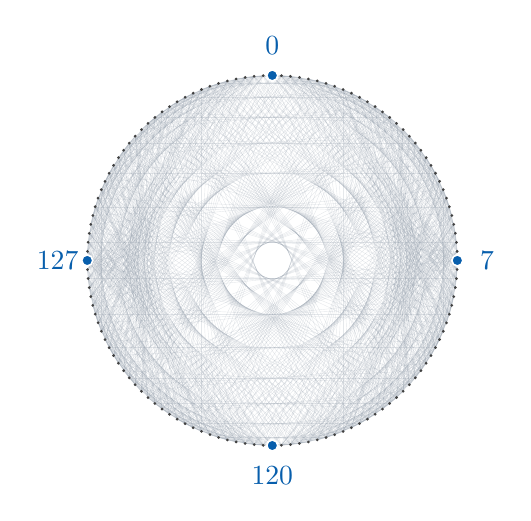
\begin{tikzpicture}[x=2.35cm,y=2.35cm]
\definecolor{graphblue}{RGB}{7,94,172}
\definecolor{graphgray}{RGB}{137,149,163}
\coordinate (v0) at (0.00000000,1.00000000);
\coordinate (v1) at (0.04906767,0.99879546);
\coordinate (v2) at (0.09801714,0.99518473);
\coordinate (v3) at (0.14673047,0.98917651);
\coordinate (v4) at (0.98917651,-0.14673047);
\coordinate (v5) at (0.99518473,-0.09801714);
\coordinate (v6) at (0.99879546,-0.04906767);
\coordinate (v7) at (1.00000000,0.00000000);
\coordinate (v8) at (0.19509032,0.98078528);
\coordinate (v9) at (0.24298018,0.97003125);
\coordinate (v10) at (0.29028468,0.95694034);
\coordinate (v11) at (0.33688985,0.94154407);
\coordinate (v12) at (0.94154407,-0.33688985);
\coordinate (v13) at (0.95694034,-0.29028468);
\coordinate (v14) at (0.97003125,-0.24298018);
\coordinate (v15) at (0.98078528,-0.19509032);
\coordinate (v16) at (0.38268343,0.92387953);
\coordinate (v17) at (0.42755509,0.90398929);
\coordinate (v18) at (0.47139674,0.88192126);
\coordinate (v19) at (0.51410274,0.85772861);
\coordinate (v20) at (0.85772861,-0.51410274);
\coordinate (v21) at (0.88192126,-0.47139674);
\coordinate (v22) at (0.90398929,-0.42755509);
\coordinate (v23) at (0.92387953,-0.38268343);
\coordinate (v24) at (0.55557023,0.83146961);
\coordinate (v25) at (0.59569930,0.80320753);
\coordinate (v26) at (0.63439328,0.77301045);
\coordinate (v27) at (0.67155895,0.74095113);
\coordinate (v28) at (0.74095113,-0.67155895);
\coordinate (v29) at (0.77301045,-0.63439328);
\coordinate (v30) at (0.80320753,-0.59569930);
\coordinate (v31) at (0.83146961,-0.55557023);
\coordinate (v32) at (0.70710678,0.70710678);
\coordinate (v33) at (0.74095113,0.67155895);
\coordinate (v34) at (0.77301045,0.63439328);
\coordinate (v35) at (0.80320753,0.59569930);
\coordinate (v36) at (0.59569930,-0.80320753);
\coordinate (v37) at (0.63439328,-0.77301045);
\coordinate (v38) at (0.67155895,-0.74095113);
\coordinate (v39) at (0.70710678,-0.70710678);
\coordinate (v40) at (0.83146961,0.55557023);
\coordinate (v41) at (0.85772861,0.51410274);
\coordinate (v42) at (0.88192126,0.47139674);
\coordinate (v43) at (0.90398929,0.42755509);
\coordinate (v44) at (0.42755509,-0.90398929);
\coordinate (v45) at (0.47139674,-0.88192126);
\coordinate (v46) at (0.51410274,-0.85772861);
\coordinate (v47) at (0.55557023,-0.83146961);
\coordinate (v48) at (0.92387953,0.38268343);
\coordinate (v49) at (0.94154407,0.33688985);
\coordinate (v50) at (0.95694034,0.29028468);
\coordinate (v51) at (0.97003125,0.24298018);
\coordinate (v52) at (0.24298018,-0.97003125);
\coordinate (v53) at (0.29028468,-0.95694034);
\coordinate (v54) at (0.33688985,-0.94154407);
\coordinate (v55) at (0.38268343,-0.92387953);
\coordinate (v56) at (0.98078528,0.19509032);
\coordinate (v57) at (0.98917651,0.14673047);
\coordinate (v58) at (0.99518473,0.09801714);
\coordinate (v59) at (0.99879546,0.04906767);
\coordinate (v60) at (0.04906767,-0.99879546);
\coordinate (v61) at (0.09801714,-0.99518473);
\coordinate (v62) at (0.14673047,-0.98917651);
\coordinate (v63) at (0.19509032,-0.98078528);
\coordinate (v64) at (-0.98078528,-0.19509032);
\coordinate (v65) at (-0.98917651,-0.14673047);
\coordinate (v66) at (-0.99518473,-0.09801714);
\coordinate (v67) at (-0.99879546,-0.04906767);
\coordinate (v68) at (-0.04906767,0.99879546);
\coordinate (v69) at (-0.09801714,0.99518473);
\coordinate (v70) at (-0.14673047,0.98917651);
\coordinate (v71) at (-0.19509032,0.98078528);
\coordinate (v72) at (-0.92387953,-0.38268343);
\coordinate (v73) at (-0.94154407,-0.33688985);
\coordinate (v74) at (-0.95694034,-0.29028468);
\coordinate (v75) at (-0.97003125,-0.24298018);
\coordinate (v76) at (-0.24298018,0.97003125);
\coordinate (v77) at (-0.29028468,0.95694034);
\coordinate (v78) at (-0.33688985,0.94154407);
\coordinate (v79) at (-0.38268343,0.92387953);
\coordinate (v80) at (-0.83146961,-0.55557023);
\coordinate (v81) at (-0.85772861,-0.51410274);
\coordinate (v82) at (-0.88192126,-0.47139674);
\coordinate (v83) at (-0.90398929,-0.42755509);
\coordinate (v84) at (-0.42755509,0.90398929);
\coordinate (v85) at (-0.47139674,0.88192126);
\coordinate (v86) at (-0.51410274,0.85772861);
\coordinate (v87) at (-0.55557023,0.83146961);
\coordinate (v88) at (-0.70710678,-0.70710678);
\coordinate (v89) at (-0.74095113,-0.67155895);
\coordinate (v90) at (-0.77301045,-0.63439328);
\coordinate (v91) at (-0.80320753,-0.59569930);
\coordinate (v92) at (-0.59569930,0.80320753);
\coordinate (v93) at (-0.63439328,0.77301045);
\coordinate (v94) at (-0.67155895,0.74095113);
\coordinate (v95) at (-0.70710678,0.70710678);
\coordinate (v96) at (-0.55557023,-0.83146961);
\coordinate (v97) at (-0.59569930,-0.80320753);
\coordinate (v98) at (-0.63439328,-0.77301045);
\coordinate (v99) at (-0.67155895,-0.74095113);
\coordinate (v100) at (-0.74095113,0.67155895);
\coordinate (v101) at (-0.77301045,0.63439328);
\coordinate (v102) at (-0.80320753,0.59569930);
\coordinate (v103) at (-0.83146961,0.55557023);
\coordinate (v104) at (-0.38268343,-0.92387953);
\coordinate (v105) at (-0.42755509,-0.90398929);
\coordinate (v106) at (-0.47139674,-0.88192126);
\coordinate (v107) at (-0.51410274,-0.85772861);
\coordinate (v108) at (-0.85772861,0.51410274);
\coordinate (v109) at (-0.88192126,0.47139674);
\coordinate (v110) at (-0.90398929,0.42755509);
\coordinate (v111) at (-0.92387953,0.38268343);
\coordinate (v112) at (-0.19509032,-0.98078528);
\coordinate (v113) at (-0.24298018,-0.97003125);
\coordinate (v114) at (-0.29028468,-0.95694034);
\coordinate (v115) at (-0.33688985,-0.94154407);
\coordinate (v116) at (-0.94154407,0.33688985);
\coordinate (v117) at (-0.95694034,0.29028468);
\coordinate (v118) at (-0.97003125,0.24298018);
\coordinate (v119) at (-0.98078528,0.19509032);
\coordinate (v120) at (0.00000000,-1.00000000);
\coordinate (v121) at (-0.04906767,-0.99879546);
\coordinate (v122) at (-0.09801714,-0.99518473);
\coordinate (v123) at (-0.14673047,-0.98917651);
\coordinate (v124) at (-0.98917651,0.14673047);
\coordinate (v125) at (-0.99518473,0.09801714);
\coordinate (v126) at (-0.99879546,0.04906767);
\coordinate (v127) at (-1.00000000,-0.00000000);
\begin{scope}[draw=graphgray,opacity=.22,line width=.15pt]
\draw (v0) -- (v1);
\draw (v0) -- (v2);
\draw (v0) -- (v3);
\draw (v0) -- (v4);
\draw (v0) -- (v5);
\draw (v0) -- (v6);
\draw (v0) -- (v8);
\draw (v0) -- (v15);
\draw (v0) -- (v16);
\draw (v0) -- (v23);
\draw (v0) -- (v24);
\draw (v0) -- (v32);
\draw (v0) -- (v39);
\draw (v0) -- (v40);
\draw (v0) -- (v48);
\draw (v0) -- (v64);
\draw (v0) -- (v71);
\draw (v0) -- (v72);
\draw (v0) -- (v80);
\draw (v0) -- (v96);
\draw (v1) -- (v3);
\draw (v1) -- (v2);
\draw (v1) -- (v5);
\draw (v1) -- (v4);
\draw (v1) -- (v7);
\draw (v1) -- (v9);
\draw (v1) -- (v14);
\draw (v1) -- (v17);
\draw (v1) -- (v22);
\draw (v1) -- (v25);
\draw (v1) -- (v33);
\draw (v1) -- (v38);
\draw (v1) -- (v41);
\draw (v1) -- (v49);
\draw (v1) -- (v65);
\draw (v1) -- (v70);
\draw (v1) -- (v73);
\draw (v1) -- (v81);
\draw (v1) -- (v97);
\draw (v2) -- (v3);
\draw (v2) -- (v6);
\draw (v2) -- (v7);
\draw (v2) -- (v4);
\draw (v2) -- (v10);
\draw (v2) -- (v13);
\draw (v2) -- (v18);
\draw (v2) -- (v21);
\draw (v2) -- (v26);
\draw (v2) -- (v34);
\draw (v2) -- (v37);
\draw (v2) -- (v42);
\draw (v2) -- (v50);
\draw (v2) -- (v66);
\draw (v2) -- (v69);
\draw (v2) -- (v74);
\draw (v2) -- (v82);
\draw (v2) -- (v98);
\draw (v3) -- (v7);
\draw (v3) -- (v6);
\draw (v3) -- (v5);
\draw (v3) -- (v11);
\draw (v3) -- (v12);
\draw (v3) -- (v19);
\draw (v3) -- (v20);
\draw (v3) -- (v27);
\draw (v3) -- (v35);
\draw (v3) -- (v36);
\draw (v3) -- (v43);
\draw (v3) -- (v51);
\draw (v3) -- (v67);
\draw (v3) -- (v68);
\draw (v3) -- (v75);
\draw (v3) -- (v83);
\draw (v3) -- (v99);
\draw (v4) -- (v5);
\draw (v4) -- (v6);
\draw (v4) -- (v7);
\draw (v4) -- (v12);
\draw (v4) -- (v11);
\draw (v4) -- (v20);
\draw (v4) -- (v19);
\draw (v4) -- (v28);
\draw (v4) -- (v36);
\draw (v4) -- (v35);
\draw (v4) -- (v44);
\draw (v4) -- (v52);
\draw (v4) -- (v68);
\draw (v4) -- (v67);
\draw (v4) -- (v76);
\draw (v4) -- (v84);
\draw (v4) -- (v100);
\draw (v5) -- (v7);
\draw (v5) -- (v6);
\draw (v5) -- (v13);
\draw (v5) -- (v10);
\draw (v5) -- (v21);
\draw (v5) -- (v18);
\draw (v5) -- (v29);
\draw (v5) -- (v37);
\draw (v5) -- (v34);
\draw (v5) -- (v45);
\draw (v5) -- (v53);
\draw (v5) -- (v69);
\draw (v5) -- (v66);
\draw (v5) -- (v77);
\draw (v5) -- (v85);
\draw (v5) -- (v101);
\draw (v6) -- (v7);
\draw (v6) -- (v14);
\draw (v6) -- (v9);
\draw (v6) -- (v22);
\draw (v6) -- (v17);
\draw (v6) -- (v30);
\draw (v6) -- (v38);
\draw (v6) -- (v33);
\draw (v6) -- (v46);
\draw (v6) -- (v54);
\draw (v6) -- (v70);
\draw (v6) -- (v65);
\draw (v6) -- (v78);
\draw (v6) -- (v86);
\draw (v6) -- (v102);
\draw (v7) -- (v15);
\draw (v7) -- (v8);
\draw (v7) -- (v23);
\draw (v7) -- (v16);
\draw (v7) -- (v31);
\draw (v7) -- (v39);
\draw (v7) -- (v32);
\draw (v7) -- (v47);
\draw (v7) -- (v55);
\draw (v7) -- (v71);
\draw (v7) -- (v64);
\draw (v7) -- (v79);
\draw (v7) -- (v87);
\draw (v7) -- (v103);
\draw (v8) -- (v9);
\draw (v8) -- (v10);
\draw (v8) -- (v11);
\draw (v8) -- (v12);
\draw (v8) -- (v13);
\draw (v8) -- (v14);
\draw (v8) -- (v24);
\draw (v8) -- (v31);
\draw (v8) -- (v16);
\draw (v8) -- (v40);
\draw (v8) -- (v47);
\draw (v8) -- (v32);
\draw (v8) -- (v56);
\draw (v8) -- (v72);
\draw (v8) -- (v79);
\draw (v8) -- (v64);
\draw (v8) -- (v88);
\draw (v8) -- (v104);
\draw (v9) -- (v11);
\draw (v9) -- (v10);
\draw (v9) -- (v13);
\draw (v9) -- (v12);
\draw (v9) -- (v15);
\draw (v9) -- (v25);
\draw (v9) -- (v30);
\draw (v9) -- (v17);
\draw (v9) -- (v41);
\draw (v9) -- (v46);
\draw (v9) -- (v33);
\draw (v9) -- (v57);
\draw (v9) -- (v73);
\draw (v9) -- (v78);
\draw (v9) -- (v65);
\draw (v9) -- (v89);
\draw (v9) -- (v105);
\draw (v10) -- (v11);
\draw (v10) -- (v14);
\draw (v10) -- (v15);
\draw (v10) -- (v12);
\draw (v10) -- (v26);
\draw (v10) -- (v29);
\draw (v10) -- (v18);
\draw (v10) -- (v42);
\draw (v10) -- (v45);
\draw (v10) -- (v34);
\draw (v10) -- (v58);
\draw (v10) -- (v74);
\draw (v10) -- (v77);
\draw (v10) -- (v66);
\draw (v10) -- (v90);
\draw (v10) -- (v106);
\draw (v11) -- (v15);
\draw (v11) -- (v14);
\draw (v11) -- (v13);
\draw (v11) -- (v27);
\draw (v11) -- (v28);
\draw (v11) -- (v19);
\draw (v11) -- (v43);
\draw (v11) -- (v44);
\draw (v11) -- (v35);
\draw (v11) -- (v59);
\draw (v11) -- (v75);
\draw (v11) -- (v76);
\draw (v11) -- (v67);
\draw (v11) -- (v91);
\draw (v11) -- (v107);
\draw (v12) -- (v13);
\draw (v12) -- (v14);
\draw (v12) -- (v15);
\draw (v12) -- (v28);
\draw (v12) -- (v27);
\draw (v12) -- (v20);
\draw (v12) -- (v44);
\draw (v12) -- (v43);
\draw (v12) -- (v36);
\draw (v12) -- (v60);
\draw (v12) -- (v76);
\draw (v12) -- (v75);
\draw (v12) -- (v68);
\draw (v12) -- (v92);
\draw (v12) -- (v108);
\draw (v13) -- (v15);
\draw (v13) -- (v14);
\draw (v13) -- (v29);
\draw (v13) -- (v26);
\draw (v13) -- (v21);
\draw (v13) -- (v45);
\draw (v13) -- (v42);
\draw (v13) -- (v37);
\draw (v13) -- (v61);
\draw (v13) -- (v77);
\draw (v13) -- (v74);
\draw (v13) -- (v69);
\draw (v13) -- (v93);
\draw (v13) -- (v109);
\draw (v14) -- (v15);
\draw (v14) -- (v30);
\draw (v14) -- (v25);
\draw (v14) -- (v22);
\draw (v14) -- (v46);
\draw (v14) -- (v41);
\draw (v14) -- (v38);
\draw (v14) -- (v62);
\draw (v14) -- (v78);
\draw (v14) -- (v73);
\draw (v14) -- (v70);
\draw (v14) -- (v94);
\draw (v14) -- (v110);
\draw (v15) -- (v31);
\draw (v15) -- (v24);
\draw (v15) -- (v23);
\draw (v15) -- (v47);
\draw (v15) -- (v40);
\draw (v15) -- (v39);
\draw (v15) -- (v63);
\draw (v15) -- (v79);
\draw (v15) -- (v72);
\draw (v15) -- (v71);
\draw (v15) -- (v95);
\draw (v15) -- (v111);
\draw (v16) -- (v17);
\draw (v16) -- (v18);
\draw (v16) -- (v19);
\draw (v16) -- (v20);
\draw (v16) -- (v21);
\draw (v16) -- (v22);
\draw (v16) -- (v24);
\draw (v16) -- (v31);
\draw (v16) -- (v48);
\draw (v16) -- (v55);
\draw (v16) -- (v56);
\draw (v16) -- (v32);
\draw (v16) -- (v80);
\draw (v16) -- (v87);
\draw (v16) -- (v88);
\draw (v16) -- (v64);
\draw (v16) -- (v112);
\draw (v17) -- (v19);
\draw (v17) -- (v18);
\draw (v17) -- (v21);
\draw (v17) -- (v20);
\draw (v17) -- (v23);
\draw (v17) -- (v25);
\draw (v17) -- (v30);
\draw (v17) -- (v49);
\draw (v17) -- (v54);
\draw (v17) -- (v57);
\draw (v17) -- (v33);
\draw (v17) -- (v81);
\draw (v17) -- (v86);
\draw (v17) -- (v89);
\draw (v17) -- (v65);
\draw (v17) -- (v113);
\draw (v18) -- (v19);
\draw (v18) -- (v22);
\draw (v18) -- (v23);
\draw (v18) -- (v20);
\draw (v18) -- (v26);
\draw (v18) -- (v29);
\draw (v18) -- (v50);
\draw (v18) -- (v53);
\draw (v18) -- (v58);
\draw (v18) -- (v34);
\draw (v18) -- (v82);
\draw (v18) -- (v85);
\draw (v18) -- (v90);
\draw (v18) -- (v66);
\draw (v18) -- (v114);
\draw (v19) -- (v23);
\draw (v19) -- (v22);
\draw (v19) -- (v21);
\draw (v19) -- (v27);
\draw (v19) -- (v28);
\draw (v19) -- (v51);
\draw (v19) -- (v52);
\draw (v19) -- (v59);
\draw (v19) -- (v35);
\draw (v19) -- (v83);
\draw (v19) -- (v84);
\draw (v19) -- (v91);
\draw (v19) -- (v67);
\draw (v19) -- (v115);
\draw (v20) -- (v21);
\draw (v20) -- (v22);
\draw (v20) -- (v23);
\draw (v20) -- (v28);
\draw (v20) -- (v27);
\draw (v20) -- (v52);
\draw (v20) -- (v51);
\draw (v20) -- (v60);
\draw (v20) -- (v36);
\draw (v20) -- (v84);
\draw (v20) -- (v83);
\draw (v20) -- (v92);
\draw (v20) -- (v68);
\draw (v20) -- (v116);
\draw (v21) -- (v23);
\draw (v21) -- (v22);
\draw (v21) -- (v29);
\draw (v21) -- (v26);
\draw (v21) -- (v53);
\draw (v21) -- (v50);
\draw (v21) -- (v61);
\draw (v21) -- (v37);
\draw (v21) -- (v85);
\draw (v21) -- (v82);
\draw (v21) -- (v93);
\draw (v21) -- (v69);
\draw (v21) -- (v117);
\draw (v22) -- (v23);
\draw (v22) -- (v30);
\draw (v22) -- (v25);
\draw (v22) -- (v54);
\draw (v22) -- (v49);
\draw (v22) -- (v62);
\draw (v22) -- (v38);
\draw (v22) -- (v86);
\draw (v22) -- (v81);
\draw (v22) -- (v94);
\draw (v22) -- (v70);
\draw (v22) -- (v118);
\draw (v23) -- (v31);
\draw (v23) -- (v24);
\draw (v23) -- (v55);
\draw (v23) -- (v48);
\draw (v23) -- (v63);
\draw (v23) -- (v39);
\draw (v23) -- (v87);
\draw (v23) -- (v80);
\draw (v23) -- (v95);
\draw (v23) -- (v71);
\draw (v23) -- (v119);
\draw (v24) -- (v25);
\draw (v24) -- (v26);
\draw (v24) -- (v27);
\draw (v24) -- (v28);
\draw (v24) -- (v29);
\draw (v24) -- (v30);
\draw (v24) -- (v56);
\draw (v24) -- (v63);
\draw (v24) -- (v48);
\draw (v24) -- (v40);
\draw (v24) -- (v88);
\draw (v24) -- (v95);
\draw (v24) -- (v80);
\draw (v24) -- (v72);
\draw (v24) -- (v120);
\draw (v25) -- (v27);
\draw (v25) -- (v26);
\draw (v25) -- (v29);
\draw (v25) -- (v28);
\draw (v25) -- (v31);
\draw (v25) -- (v57);
\draw (v25) -- (v62);
\draw (v25) -- (v49);
\draw (v25) -- (v41);
\draw (v25) -- (v89);
\draw (v25) -- (v94);
\draw (v25) -- (v81);
\draw (v25) -- (v73);
\draw (v25) -- (v121);
\draw (v26) -- (v27);
\draw (v26) -- (v30);
\draw (v26) -- (v31);
\draw (v26) -- (v28);
\draw (v26) -- (v58);
\draw (v26) -- (v61);
\draw (v26) -- (v50);
\draw (v26) -- (v42);
\draw (v26) -- (v90);
\draw (v26) -- (v93);
\draw (v26) -- (v82);
\draw (v26) -- (v74);
\draw (v26) -- (v122);
\draw (v27) -- (v31);
\draw (v27) -- (v30);
\draw (v27) -- (v29);
\draw (v27) -- (v59);
\draw (v27) -- (v60);
\draw (v27) -- (v51);
\draw (v27) -- (v43);
\draw (v27) -- (v91);
\draw (v27) -- (v92);
\draw (v27) -- (v83);
\draw (v27) -- (v75);
\draw (v27) -- (v123);
\draw (v28) -- (v29);
\draw (v28) -- (v30);
\draw (v28) -- (v31);
\draw (v28) -- (v60);
\draw (v28) -- (v59);
\draw (v28) -- (v52);
\draw (v28) -- (v44);
\draw (v28) -- (v92);
\draw (v28) -- (v91);
\draw (v28) -- (v84);
\draw (v28) -- (v76);
\draw (v28) -- (v124);
\draw (v29) -- (v31);
\draw (v29) -- (v30);
\draw (v29) -- (v61);
\draw (v29) -- (v58);
\draw (v29) -- (v53);
\draw (v29) -- (v45);
\draw (v29) -- (v93);
\draw (v29) -- (v90);
\draw (v29) -- (v85);
\draw (v29) -- (v77);
\draw (v29) -- (v125);
\draw (v30) -- (v31);
\draw (v30) -- (v62);
\draw (v30) -- (v57);
\draw (v30) -- (v54);
\draw (v30) -- (v46);
\draw (v30) -- (v94);
\draw (v30) -- (v89);
\draw (v30) -- (v86);
\draw (v30) -- (v78);
\draw (v30) -- (v126);
\draw (v31) -- (v63);
\draw (v31) -- (v56);
\draw (v31) -- (v55);
\draw (v31) -- (v47);
\draw (v31) -- (v95);
\draw (v31) -- (v88);
\draw (v31) -- (v87);
\draw (v31) -- (v79);
\draw (v31) -- (v127);
\draw (v32) -- (v33);
\draw (v32) -- (v34);
\draw (v32) -- (v35);
\draw (v32) -- (v36);
\draw (v32) -- (v37);
\draw (v32) -- (v38);
\draw (v32) -- (v40);
\draw (v32) -- (v47);
\draw (v32) -- (v48);
\draw (v32) -- (v55);
\draw (v32) -- (v56);
\draw (v32) -- (v96);
\draw (v32) -- (v103);
\draw (v32) -- (v104);
\draw (v32) -- (v112);
\draw (v32) -- (v64);
\draw (v33) -- (v35);
\draw (v33) -- (v34);
\draw (v33) -- (v37);
\draw (v33) -- (v36);
\draw (v33) -- (v39);
\draw (v33) -- (v41);
\draw (v33) -- (v46);
\draw (v33) -- (v49);
\draw (v33) -- (v54);
\draw (v33) -- (v57);
\draw (v33) -- (v97);
\draw (v33) -- (v102);
\draw (v33) -- (v105);
\draw (v33) -- (v113);
\draw (v33) -- (v65);
\draw (v34) -- (v35);
\draw (v34) -- (v38);
\draw (v34) -- (v39);
\draw (v34) -- (v36);
\draw (v34) -- (v42);
\draw (v34) -- (v45);
\draw (v34) -- (v50);
\draw (v34) -- (v53);
\draw (v34) -- (v58);
\draw (v34) -- (v98);
\draw (v34) -- (v101);
\draw (v34) -- (v106);
\draw (v34) -- (v114);
\draw (v34) -- (v66);
\draw (v35) -- (v39);
\draw (v35) -- (v38);
\draw (v35) -- (v37);
\draw (v35) -- (v43);
\draw (v35) -- (v44);
\draw (v35) -- (v51);
\draw (v35) -- (v52);
\draw (v35) -- (v59);
\draw (v35) -- (v99);
\draw (v35) -- (v100);
\draw (v35) -- (v107);
\draw (v35) -- (v115);
\draw (v35) -- (v67);
\draw (v36) -- (v37);
\draw (v36) -- (v38);
\draw (v36) -- (v39);
\draw (v36) -- (v44);
\draw (v36) -- (v43);
\draw (v36) -- (v52);
\draw (v36) -- (v51);
\draw (v36) -- (v60);
\draw (v36) -- (v100);
\draw (v36) -- (v99);
\draw (v36) -- (v108);
\draw (v36) -- (v116);
\draw (v36) -- (v68);
\draw (v37) -- (v39);
\draw (v37) -- (v38);
\draw (v37) -- (v45);
\draw (v37) -- (v42);
\draw (v37) -- (v53);
\draw (v37) -- (v50);
\draw (v37) -- (v61);
\draw (v37) -- (v101);
\draw (v37) -- (v98);
\draw (v37) -- (v109);
\draw (v37) -- (v117);
\draw (v37) -- (v69);
\draw (v38) -- (v39);
\draw (v38) -- (v46);
\draw (v38) -- (v41);
\draw (v38) -- (v54);
\draw (v38) -- (v49);
\draw (v38) -- (v62);
\draw (v38) -- (v102);
\draw (v38) -- (v97);
\draw (v38) -- (v110);
\draw (v38) -- (v118);
\draw (v38) -- (v70);
\draw (v39) -- (v47);
\draw (v39) -- (v40);
\draw (v39) -- (v55);
\draw (v39) -- (v48);
\draw (v39) -- (v63);
\draw (v39) -- (v103);
\draw (v39) -- (v96);
\draw (v39) -- (v111);
\draw (v39) -- (v119);
\draw (v39) -- (v71);
\draw (v40) -- (v41);
\draw (v40) -- (v42);
\draw (v40) -- (v43);
\draw (v40) -- (v44);
\draw (v40) -- (v45);
\draw (v40) -- (v46);
\draw (v40) -- (v56);
\draw (v40) -- (v63);
\draw (v40) -- (v48);
\draw (v40) -- (v104);
\draw (v40) -- (v111);
\draw (v40) -- (v96);
\draw (v40) -- (v120);
\draw (v40) -- (v72);
\draw (v41) -- (v43);
\draw (v41) -- (v42);
\draw (v41) -- (v45);
\draw (v41) -- (v44);
\draw (v41) -- (v47);
\draw (v41) -- (v57);
\draw (v41) -- (v62);
\draw (v41) -- (v49);
\draw (v41) -- (v105);
\draw (v41) -- (v110);
\draw (v41) -- (v97);
\draw (v41) -- (v121);
\draw (v41) -- (v73);
\draw (v42) -- (v43);
\draw (v42) -- (v46);
\draw (v42) -- (v47);
\draw (v42) -- (v44);
\draw (v42) -- (v58);
\draw (v42) -- (v61);
\draw (v42) -- (v50);
\draw (v42) -- (v106);
\draw (v42) -- (v109);
\draw (v42) -- (v98);
\draw (v42) -- (v122);
\draw (v42) -- (v74);
\draw (v43) -- (v47);
\draw (v43) -- (v46);
\draw (v43) -- (v45);
\draw (v43) -- (v59);
\draw (v43) -- (v60);
\draw (v43) -- (v51);
\draw (v43) -- (v107);
\draw (v43) -- (v108);
\draw (v43) -- (v99);
\draw (v43) -- (v123);
\draw (v43) -- (v75);
\draw (v44) -- (v45);
\draw (v44) -- (v46);
\draw (v44) -- (v47);
\draw (v44) -- (v60);
\draw (v44) -- (v59);
\draw (v44) -- (v52);
\draw (v44) -- (v108);
\draw (v44) -- (v107);
\draw (v44) -- (v100);
\draw (v44) -- (v124);
\draw (v44) -- (v76);
\draw (v45) -- (v47);
\draw (v45) -- (v46);
\draw (v45) -- (v61);
\draw (v45) -- (v58);
\draw (v45) -- (v53);
\draw (v45) -- (v109);
\draw (v45) -- (v106);
\draw (v45) -- (v101);
\draw (v45) -- (v125);
\draw (v45) -- (v77);
\draw (v46) -- (v47);
\draw (v46) -- (v62);
\draw (v46) -- (v57);
\draw (v46) -- (v54);
\draw (v46) -- (v110);
\draw (v46) -- (v105);
\draw (v46) -- (v102);
\draw (v46) -- (v126);
\draw (v46) -- (v78);
\draw (v47) -- (v63);
\draw (v47) -- (v56);
\draw (v47) -- (v55);
\draw (v47) -- (v111);
\draw (v47) -- (v104);
\draw (v47) -- (v103);
\draw (v47) -- (v127);
\draw (v47) -- (v79);
\draw (v48) -- (v49);
\draw (v48) -- (v50);
\draw (v48) -- (v51);
\draw (v48) -- (v52);
\draw (v48) -- (v53);
\draw (v48) -- (v54);
\draw (v48) -- (v56);
\draw (v48) -- (v63);
\draw (v48) -- (v112);
\draw (v48) -- (v119);
\draw (v48) -- (v120);
\draw (v48) -- (v96);
\draw (v48) -- (v80);
\draw (v49) -- (v51);
\draw (v49) -- (v50);
\draw (v49) -- (v53);
\draw (v49) -- (v52);
\draw (v49) -- (v55);
\draw (v49) -- (v57);
\draw (v49) -- (v62);
\draw (v49) -- (v113);
\draw (v49) -- (v118);
\draw (v49) -- (v121);
\draw (v49) -- (v97);
\draw (v49) -- (v81);
\draw (v50) -- (v51);
\draw (v50) -- (v54);
\draw (v50) -- (v55);
\draw (v50) -- (v52);
\draw (v50) -- (v58);
\draw (v50) -- (v61);
\draw (v50) -- (v114);
\draw (v50) -- (v117);
\draw (v50) -- (v122);
\draw (v50) -- (v98);
\draw (v50) -- (v82);
\draw (v51) -- (v55);
\draw (v51) -- (v54);
\draw (v51) -- (v53);
\draw (v51) -- (v59);
\draw (v51) -- (v60);
\draw (v51) -- (v115);
\draw (v51) -- (v116);
\draw (v51) -- (v123);
\draw (v51) -- (v99);
\draw (v51) -- (v83);
\draw (v52) -- (v53);
\draw (v52) -- (v54);
\draw (v52) -- (v55);
\draw (v52) -- (v60);
\draw (v52) -- (v59);
\draw (v52) -- (v116);
\draw (v52) -- (v115);
\draw (v52) -- (v124);
\draw (v52) -- (v100);
\draw (v52) -- (v84);
\draw (v53) -- (v55);
\draw (v53) -- (v54);
\draw (v53) -- (v61);
\draw (v53) -- (v58);
\draw (v53) -- (v117);
\draw (v53) -- (v114);
\draw (v53) -- (v125);
\draw (v53) -- (v101);
\draw (v53) -- (v85);
\draw (v54) -- (v55);
\draw (v54) -- (v62);
\draw (v54) -- (v57);
\draw (v54) -- (v118);
\draw (v54) -- (v113);
\draw (v54) -- (v126);
\draw (v54) -- (v102);
\draw (v54) -- (v86);
\draw (v55) -- (v63);
\draw (v55) -- (v56);
\draw (v55) -- (v119);
\draw (v55) -- (v112);
\draw (v55) -- (v127);
\draw (v55) -- (v103);
\draw (v55) -- (v87);
\draw (v56) -- (v57);
\draw (v56) -- (v58);
\draw (v56) -- (v59);
\draw (v56) -- (v60);
\draw (v56) -- (v61);
\draw (v56) -- (v62);
\draw (v56) -- (v120);
\draw (v56) -- (v127);
\draw (v56) -- (v112);
\draw (v56) -- (v104);
\draw (v56) -- (v88);
\draw (v57) -- (v59);
\draw (v57) -- (v58);
\draw (v57) -- (v61);
\draw (v57) -- (v60);
\draw (v57) -- (v63);
\draw (v57) -- (v121);
\draw (v57) -- (v126);
\draw (v57) -- (v113);
\draw (v57) -- (v105);
\draw (v57) -- (v89);
\draw (v58) -- (v59);
\draw (v58) -- (v62);
\draw (v58) -- (v63);
\draw (v58) -- (v60);
\draw (v58) -- (v122);
\draw (v58) -- (v125);
\draw (v58) -- (v114);
\draw (v58) -- (v106);
\draw (v58) -- (v90);
\draw (v59) -- (v63);
\draw (v59) -- (v62);
\draw (v59) -- (v61);
\draw (v59) -- (v123);
\draw (v59) -- (v124);
\draw (v59) -- (v115);
\draw (v59) -- (v107);
\draw (v59) -- (v91);
\draw (v60) -- (v61);
\draw (v60) -- (v62);
\draw (v60) -- (v63);
\draw (v60) -- (v124);
\draw (v60) -- (v123);
\draw (v60) -- (v116);
\draw (v60) -- (v108);
\draw (v60) -- (v92);
\draw (v61) -- (v63);
\draw (v61) -- (v62);
\draw (v61) -- (v125);
\draw (v61) -- (v122);
\draw (v61) -- (v117);
\draw (v61) -- (v109);
\draw (v61) -- (v93);
\draw (v62) -- (v63);
\draw (v62) -- (v126);
\draw (v62) -- (v121);
\draw (v62) -- (v118);
\draw (v62) -- (v110);
\draw (v62) -- (v94);
\draw (v63) -- (v127);
\draw (v63) -- (v120);
\draw (v63) -- (v119);
\draw (v63) -- (v111);
\draw (v63) -- (v95);
\draw (v64) -- (v65);
\draw (v64) -- (v66);
\draw (v64) -- (v67);
\draw (v64) -- (v68);
\draw (v64) -- (v69);
\draw (v64) -- (v70);
\draw (v64) -- (v72);
\draw (v64) -- (v79);
\draw (v64) -- (v80);
\draw (v64) -- (v87);
\draw (v64) -- (v88);
\draw (v64) -- (v96);
\draw (v64) -- (v103);
\draw (v64) -- (v104);
\draw (v64) -- (v112);
\draw (v65) -- (v67);
\draw (v65) -- (v66);
\draw (v65) -- (v69);
\draw (v65) -- (v68);
\draw (v65) -- (v71);
\draw (v65) -- (v73);
\draw (v65) -- (v78);
\draw (v65) -- (v81);
\draw (v65) -- (v86);
\draw (v65) -- (v89);
\draw (v65) -- (v97);
\draw (v65) -- (v102);
\draw (v65) -- (v105);
\draw (v65) -- (v113);
\draw (v66) -- (v67);
\draw (v66) -- (v70);
\draw (v66) -- (v71);
\draw (v66) -- (v68);
\draw (v66) -- (v74);
\draw (v66) -- (v77);
\draw (v66) -- (v82);
\draw (v66) -- (v85);
\draw (v66) -- (v90);
\draw (v66) -- (v98);
\draw (v66) -- (v101);
\draw (v66) -- (v106);
\draw (v66) -- (v114);
\draw (v67) -- (v71);
\draw (v67) -- (v70);
\draw (v67) -- (v69);
\draw (v67) -- (v75);
\draw (v67) -- (v76);
\draw (v67) -- (v83);
\draw (v67) -- (v84);
\draw (v67) -- (v91);
\draw (v67) -- (v99);
\draw (v67) -- (v100);
\draw (v67) -- (v107);
\draw (v67) -- (v115);
\draw (v68) -- (v69);
\draw (v68) -- (v70);
\draw (v68) -- (v71);
\draw (v68) -- (v76);
\draw (v68) -- (v75);
\draw (v68) -- (v84);
\draw (v68) -- (v83);
\draw (v68) -- (v92);
\draw (v68) -- (v100);
\draw (v68) -- (v99);
\draw (v68) -- (v108);
\draw (v68) -- (v116);
\draw (v69) -- (v71);
\draw (v69) -- (v70);
\draw (v69) -- (v77);
\draw (v69) -- (v74);
\draw (v69) -- (v85);
\draw (v69) -- (v82);
\draw (v69) -- (v93);
\draw (v69) -- (v101);
\draw (v69) -- (v98);
\draw (v69) -- (v109);
\draw (v69) -- (v117);
\draw (v70) -- (v71);
\draw (v70) -- (v78);
\draw (v70) -- (v73);
\draw (v70) -- (v86);
\draw (v70) -- (v81);
\draw (v70) -- (v94);
\draw (v70) -- (v102);
\draw (v70) -- (v97);
\draw (v70) -- (v110);
\draw (v70) -- (v118);
\draw (v71) -- (v79);
\draw (v71) -- (v72);
\draw (v71) -- (v87);
\draw (v71) -- (v80);
\draw (v71) -- (v95);
\draw (v71) -- (v103);
\draw (v71) -- (v96);
\draw (v71) -- (v111);
\draw (v71) -- (v119);
\draw (v72) -- (v73);
\draw (v72) -- (v74);
\draw (v72) -- (v75);
\draw (v72) -- (v76);
\draw (v72) -- (v77);
\draw (v72) -- (v78);
\draw (v72) -- (v88);
\draw (v72) -- (v95);
\draw (v72) -- (v80);
\draw (v72) -- (v104);
\draw (v72) -- (v111);
\draw (v72) -- (v96);
\draw (v72) -- (v120);
\draw (v73) -- (v75);
\draw (v73) -- (v74);
\draw (v73) -- (v77);
\draw (v73) -- (v76);
\draw (v73) -- (v79);
\draw (v73) -- (v89);
\draw (v73) -- (v94);
\draw (v73) -- (v81);
\draw (v73) -- (v105);
\draw (v73) -- (v110);
\draw (v73) -- (v97);
\draw (v73) -- (v121);
\draw (v74) -- (v75);
\draw (v74) -- (v78);
\draw (v74) -- (v79);
\draw (v74) -- (v76);
\draw (v74) -- (v90);
\draw (v74) -- (v93);
\draw (v74) -- (v82);
\draw (v74) -- (v106);
\draw (v74) -- (v109);
\draw (v74) -- (v98);
\draw (v74) -- (v122);
\draw (v75) -- (v79);
\draw (v75) -- (v78);
\draw (v75) -- (v77);
\draw (v75) -- (v91);
\draw (v75) -- (v92);
\draw (v75) -- (v83);
\draw (v75) -- (v107);
\draw (v75) -- (v108);
\draw (v75) -- (v99);
\draw (v75) -- (v123);
\draw (v76) -- (v77);
\draw (v76) -- (v78);
\draw (v76) -- (v79);
\draw (v76) -- (v92);
\draw (v76) -- (v91);
\draw (v76) -- (v84);
\draw (v76) -- (v108);
\draw (v76) -- (v107);
\draw (v76) -- (v100);
\draw (v76) -- (v124);
\draw (v77) -- (v79);
\draw (v77) -- (v78);
\draw (v77) -- (v93);
\draw (v77) -- (v90);
\draw (v77) -- (v85);
\draw (v77) -- (v109);
\draw (v77) -- (v106);
\draw (v77) -- (v101);
\draw (v77) -- (v125);
\draw (v78) -- (v79);
\draw (v78) -- (v94);
\draw (v78) -- (v89);
\draw (v78) -- (v86);
\draw (v78) -- (v110);
\draw (v78) -- (v105);
\draw (v78) -- (v102);
\draw (v78) -- (v126);
\draw (v79) -- (v95);
\draw (v79) -- (v88);
\draw (v79) -- (v87);
\draw (v79) -- (v111);
\draw (v79) -- (v104);
\draw (v79) -- (v103);
\draw (v79) -- (v127);
\draw (v80) -- (v81);
\draw (v80) -- (v82);
\draw (v80) -- (v83);
\draw (v80) -- (v84);
\draw (v80) -- (v85);
\draw (v80) -- (v86);
\draw (v80) -- (v88);
\draw (v80) -- (v95);
\draw (v80) -- (v112);
\draw (v80) -- (v119);
\draw (v80) -- (v120);
\draw (v80) -- (v96);
\draw (v81) -- (v83);
\draw (v81) -- (v82);
\draw (v81) -- (v85);
\draw (v81) -- (v84);
\draw (v81) -- (v87);
\draw (v81) -- (v89);
\draw (v81) -- (v94);
\draw (v81) -- (v113);
\draw (v81) -- (v118);
\draw (v81) -- (v121);
\draw (v81) -- (v97);
\draw (v82) -- (v83);
\draw (v82) -- (v86);
\draw (v82) -- (v87);
\draw (v82) -- (v84);
\draw (v82) -- (v90);
\draw (v82) -- (v93);
\draw (v82) -- (v114);
\draw (v82) -- (v117);
\draw (v82) -- (v122);
\draw (v82) -- (v98);
\draw (v83) -- (v87);
\draw (v83) -- (v86);
\draw (v83) -- (v85);
\draw (v83) -- (v91);
\draw (v83) -- (v92);
\draw (v83) -- (v115);
\draw (v83) -- (v116);
\draw (v83) -- (v123);
\draw (v83) -- (v99);
\draw (v84) -- (v85);
\draw (v84) -- (v86);
\draw (v84) -- (v87);
\draw (v84) -- (v92);
\draw (v84) -- (v91);
\draw (v84) -- (v116);
\draw (v84) -- (v115);
\draw (v84) -- (v124);
\draw (v84) -- (v100);
\draw (v85) -- (v87);
\draw (v85) -- (v86);
\draw (v85) -- (v93);
\draw (v85) -- (v90);
\draw (v85) -- (v117);
\draw (v85) -- (v114);
\draw (v85) -- (v125);
\draw (v85) -- (v101);
\draw (v86) -- (v87);
\draw (v86) -- (v94);
\draw (v86) -- (v89);
\draw (v86) -- (v118);
\draw (v86) -- (v113);
\draw (v86) -- (v126);
\draw (v86) -- (v102);
\draw (v87) -- (v95);
\draw (v87) -- (v88);
\draw (v87) -- (v119);
\draw (v87) -- (v112);
\draw (v87) -- (v127);
\draw (v87) -- (v103);
\draw (v88) -- (v89);
\draw (v88) -- (v90);
\draw (v88) -- (v91);
\draw (v88) -- (v92);
\draw (v88) -- (v93);
\draw (v88) -- (v94);
\draw (v88) -- (v120);
\draw (v88) -- (v127);
\draw (v88) -- (v112);
\draw (v88) -- (v104);
\draw (v89) -- (v91);
\draw (v89) -- (v90);
\draw (v89) -- (v93);
\draw (v89) -- (v92);
\draw (v89) -- (v95);
\draw (v89) -- (v121);
\draw (v89) -- (v126);
\draw (v89) -- (v113);
\draw (v89) -- (v105);
\draw (v90) -- (v91);
\draw (v90) -- (v94);
\draw (v90) -- (v95);
\draw (v90) -- (v92);
\draw (v90) -- (v122);
\draw (v90) -- (v125);
\draw (v90) -- (v114);
\draw (v90) -- (v106);
\draw (v91) -- (v95);
\draw (v91) -- (v94);
\draw (v91) -- (v93);
\draw (v91) -- (v123);
\draw (v91) -- (v124);
\draw (v91) -- (v115);
\draw (v91) -- (v107);
\draw (v92) -- (v93);
\draw (v92) -- (v94);
\draw (v92) -- (v95);
\draw (v92) -- (v124);
\draw (v92) -- (v123);
\draw (v92) -- (v116);
\draw (v92) -- (v108);
\draw (v93) -- (v95);
\draw (v93) -- (v94);
\draw (v93) -- (v125);
\draw (v93) -- (v122);
\draw (v93) -- (v117);
\draw (v93) -- (v109);
\draw (v94) -- (v95);
\draw (v94) -- (v126);
\draw (v94) -- (v121);
\draw (v94) -- (v118);
\draw (v94) -- (v110);
\draw (v95) -- (v127);
\draw (v95) -- (v120);
\draw (v95) -- (v119);
\draw (v95) -- (v111);
\draw (v96) -- (v97);
\draw (v96) -- (v98);
\draw (v96) -- (v99);
\draw (v96) -- (v100);
\draw (v96) -- (v101);
\draw (v96) -- (v102);
\draw (v96) -- (v104);
\draw (v96) -- (v111);
\draw (v96) -- (v112);
\draw (v96) -- (v119);
\draw (v96) -- (v120);
\draw (v97) -- (v99);
\draw (v97) -- (v98);
\draw (v97) -- (v101);
\draw (v97) -- (v100);
\draw (v97) -- (v103);
\draw (v97) -- (v105);
\draw (v97) -- (v110);
\draw (v97) -- (v113);
\draw (v97) -- (v118);
\draw (v97) -- (v121);
\draw (v98) -- (v99);
\draw (v98) -- (v102);
\draw (v98) -- (v103);
\draw (v98) -- (v100);
\draw (v98) -- (v106);
\draw (v98) -- (v109);
\draw (v98) -- (v114);
\draw (v98) -- (v117);
\draw (v98) -- (v122);
\draw (v99) -- (v103);
\draw (v99) -- (v102);
\draw (v99) -- (v101);
\draw (v99) -- (v107);
\draw (v99) -- (v108);
\draw (v99) -- (v115);
\draw (v99) -- (v116);
\draw (v99) -- (v123);
\draw (v100) -- (v101);
\draw (v100) -- (v102);
\draw (v100) -- (v103);
\draw (v100) -- (v108);
\draw (v100) -- (v107);
\draw (v100) -- (v116);
\draw (v100) -- (v115);
\draw (v100) -- (v124);
\draw (v101) -- (v103);
\draw (v101) -- (v102);
\draw (v101) -- (v109);
\draw (v101) -- (v106);
\draw (v101) -- (v117);
\draw (v101) -- (v114);
\draw (v101) -- (v125);
\draw (v102) -- (v103);
\draw (v102) -- (v110);
\draw (v102) -- (v105);
\draw (v102) -- (v118);
\draw (v102) -- (v113);
\draw (v102) -- (v126);
\draw (v103) -- (v111);
\draw (v103) -- (v104);
\draw (v103) -- (v119);
\draw (v103) -- (v112);
\draw (v103) -- (v127);
\draw (v104) -- (v105);
\draw (v104) -- (v106);
\draw (v104) -- (v107);
\draw (v104) -- (v108);
\draw (v104) -- (v109);
\draw (v104) -- (v110);
\draw (v104) -- (v120);
\draw (v104) -- (v127);
\draw (v104) -- (v112);
\draw (v105) -- (v107);
\draw (v105) -- (v106);
\draw (v105) -- (v109);
\draw (v105) -- (v108);
\draw (v105) -- (v111);
\draw (v105) -- (v121);
\draw (v105) -- (v126);
\draw (v105) -- (v113);
\draw (v106) -- (v107);
\draw (v106) -- (v110);
\draw (v106) -- (v111);
\draw (v106) -- (v108);
\draw (v106) -- (v122);
\draw (v106) -- (v125);
\draw (v106) -- (v114);
\draw (v107) -- (v111);
\draw (v107) -- (v110);
\draw (v107) -- (v109);
\draw (v107) -- (v123);
\draw (v107) -- (v124);
\draw (v107) -- (v115);
\draw (v108) -- (v109);
\draw (v108) -- (v110);
\draw (v108) -- (v111);
\draw (v108) -- (v124);
\draw (v108) -- (v123);
\draw (v108) -- (v116);
\draw (v109) -- (v111);
\draw (v109) -- (v110);
\draw (v109) -- (v125);
\draw (v109) -- (v122);
\draw (v109) -- (v117);
\draw (v110) -- (v111);
\draw (v110) -- (v126);
\draw (v110) -- (v121);
\draw (v110) -- (v118);
\draw (v111) -- (v127);
\draw (v111) -- (v120);
\draw (v111) -- (v119);
\draw (v112) -- (v113);
\draw (v112) -- (v114);
\draw (v112) -- (v115);
\draw (v112) -- (v116);
\draw (v112) -- (v117);
\draw (v112) -- (v118);
\draw (v112) -- (v120);
\draw (v112) -- (v127);
\draw (v113) -- (v115);
\draw (v113) -- (v114);
\draw (v113) -- (v117);
\draw (v113) -- (v116);
\draw (v113) -- (v119);
\draw (v113) -- (v121);
\draw (v113) -- (v126);
\draw (v114) -- (v115);
\draw (v114) -- (v118);
\draw (v114) -- (v119);
\draw (v114) -- (v116);
\draw (v114) -- (v122);
\draw (v114) -- (v125);
\draw (v115) -- (v119);
\draw (v115) -- (v118);
\draw (v115) -- (v117);
\draw (v115) -- (v123);
\draw (v115) -- (v124);
\draw (v116) -- (v117);
\draw (v116) -- (v118);
\draw (v116) -- (v119);
\draw (v116) -- (v124);
\draw (v116) -- (v123);
\draw (v117) -- (v119);
\draw (v117) -- (v118);
\draw (v117) -- (v125);
\draw (v117) -- (v122);
\draw (v118) -- (v119);
\draw (v118) -- (v126);
\draw (v118) -- (v121);
\draw (v119) -- (v127);
\draw (v119) -- (v120);
\draw (v120) -- (v121);
\draw (v120) -- (v122);
\draw (v120) -- (v123);
\draw (v120) -- (v124);
\draw (v120) -- (v125);
\draw (v120) -- (v126);
\draw (v121) -- (v123);
\draw (v121) -- (v122);
\draw (v121) -- (v125);
\draw (v121) -- (v124);
\draw (v121) -- (v127);
\draw (v122) -- (v123);
\draw (v122) -- (v126);
\draw (v122) -- (v127);
\draw (v122) -- (v124);
\draw (v123) -- (v127);
\draw (v123) -- (v126);
\draw (v123) -- (v125);
\draw (v124) -- (v125);
\draw (v124) -- (v126);
\draw (v124) -- (v127);
\draw (v125) -- (v127);
\draw (v125) -- (v126);
\draw (v126) -- (v127);
\end{scope}
\fill[black!75] (v1) circle[radius=.55pt];
\fill[black!75] (v2) circle[radius=.55pt];
\fill[black!75] (v3) circle[radius=.55pt];
\fill[black!75] (v4) circle[radius=.55pt];
\fill[black!75] (v5) circle[radius=.55pt];
\fill[black!75] (v6) circle[radius=.55pt];
\fill[black!75] (v8) circle[radius=.55pt];
\fill[black!75] (v9) circle[radius=.55pt];
\fill[black!75] (v10) circle[radius=.55pt];
\fill[black!75] (v11) circle[radius=.55pt];
\fill[black!75] (v12) circle[radius=.55pt];
\fill[black!75] (v13) circle[radius=.55pt];
\fill[black!75] (v14) circle[radius=.55pt];
\fill[black!75] (v15) circle[radius=.55pt];
\fill[black!75] (v16) circle[radius=.55pt];
\fill[black!75] (v17) circle[radius=.55pt];
\fill[black!75] (v18) circle[radius=.55pt];
\fill[black!75] (v19) circle[radius=.55pt];
\fill[black!75] (v20) circle[radius=.55pt];
\fill[black!75] (v21) circle[radius=.55pt];
\fill[black!75] (v22) circle[radius=.55pt];
\fill[black!75] (v23) circle[radius=.55pt];
\fill[black!75] (v24) circle[radius=.55pt];
\fill[black!75] (v25) circle[radius=.55pt];
\fill[black!75] (v26) circle[radius=.55pt];
\fill[black!75] (v27) circle[radius=.55pt];
\fill[black!75] (v28) circle[radius=.55pt];
\fill[black!75] (v29) circle[radius=.55pt];
\fill[black!75] (v30) circle[radius=.55pt];
\fill[black!75] (v31) circle[radius=.55pt];
\fill[black!75] (v32) circle[radius=.55pt];
\fill[black!75] (v33) circle[radius=.55pt];
\fill[black!75] (v34) circle[radius=.55pt];
\fill[black!75] (v35) circle[radius=.55pt];
\fill[black!75] (v36) circle[radius=.55pt];
\fill[black!75] (v37) circle[radius=.55pt];
\fill[black!75] (v38) circle[radius=.55pt];
\fill[black!75] (v39) circle[radius=.55pt];
\fill[black!75] (v40) circle[radius=.55pt];
\fill[black!75] (v41) circle[radius=.55pt];
\fill[black!75] (v42) circle[radius=.55pt];
\fill[black!75] (v43) circle[radius=.55pt];
\fill[black!75] (v44) circle[radius=.55pt];
\fill[black!75] (v45) circle[radius=.55pt];
\fill[black!75] (v46) circle[radius=.55pt];
\fill[black!75] (v47) circle[radius=.55pt];
\fill[black!75] (v48) circle[radius=.55pt];
\fill[black!75] (v49) circle[radius=.55pt];
\fill[black!75] (v50) circle[radius=.55pt];
\fill[black!75] (v51) circle[radius=.55pt];
\fill[black!75] (v52) circle[radius=.55pt];
\fill[black!75] (v53) circle[radius=.55pt];
\fill[black!75] (v54) circle[radius=.55pt];
\fill[black!75] (v55) circle[radius=.55pt];
\fill[black!75] (v56) circle[radius=.55pt];
\fill[black!75] (v57) circle[radius=.55pt];
\fill[black!75] (v58) circle[radius=.55pt];
\fill[black!75] (v59) circle[radius=.55pt];
\fill[black!75] (v60) circle[radius=.55pt];
\fill[black!75] (v61) circle[radius=.55pt];
\fill[black!75] (v62) circle[radius=.55pt];
\fill[black!75] (v63) circle[radius=.55pt];
\fill[black!75] (v64) circle[radius=.55pt];
\fill[black!75] (v65) circle[radius=.55pt];
\fill[black!75] (v66) circle[radius=.55pt];
\fill[black!75] (v67) circle[radius=.55pt];
\fill[black!75] (v68) circle[radius=.55pt];
\fill[black!75] (v69) circle[radius=.55pt];
\fill[black!75] (v70) circle[radius=.55pt];
\fill[black!75] (v71) circle[radius=.55pt];
\fill[black!75] (v72) circle[radius=.55pt];
\fill[black!75] (v73) circle[radius=.55pt];
\fill[black!75] (v74) circle[radius=.55pt];
\fill[black!75] (v75) circle[radius=.55pt];
\fill[black!75] (v76) circle[radius=.55pt];
\fill[black!75] (v77) circle[radius=.55pt];
\fill[black!75] (v78) circle[radius=.55pt];
\fill[black!75] (v79) circle[radius=.55pt];
\fill[black!75] (v80) circle[radius=.55pt];
\fill[black!75] (v81) circle[radius=.55pt];
\fill[black!75] (v82) circle[radius=.55pt];
\fill[black!75] (v83) circle[radius=.55pt];
\fill[black!75] (v84) circle[radius=.55pt];
\fill[black!75] (v85) circle[radius=.55pt];
\fill[black!75] (v86) circle[radius=.55pt];
\fill[black!75] (v87) circle[radius=.55pt];
\fill[black!75] (v88) circle[radius=.55pt];
\fill[black!75] (v89) circle[radius=.55pt];
\fill[black!75] (v90) circle[radius=.55pt];
\fill[black!75] (v91) circle[radius=.55pt];
\fill[black!75] (v92) circle[radius=.55pt];
\fill[black!75] (v93) circle[radius=.55pt];
\fill[black!75] (v94) circle[radius=.55pt];
\fill[black!75] (v95) circle[radius=.55pt];
\fill[black!75] (v96) circle[radius=.55pt];
\fill[black!75] (v97) circle[radius=.55pt];
\fill[black!75] (v98) circle[radius=.55pt];
\fill[black!75] (v99) circle[radius=.55pt];
\fill[black!75] (v100) circle[radius=.55pt];
\fill[black!75] (v101) circle[radius=.55pt];
\fill[black!75] (v102) circle[radius=.55pt];
\fill[black!75] (v103) circle[radius=.55pt];
\fill[black!75] (v104) circle[radius=.55pt];
\fill[black!75] (v105) circle[radius=.55pt];
\fill[black!75] (v106) circle[radius=.55pt];
\fill[black!75] (v107) circle[radius=.55pt];
\fill[black!75] (v108) circle[radius=.55pt];
\fill[black!75] (v109) circle[radius=.55pt];
\fill[black!75] (v110) circle[radius=.55pt];
\fill[black!75] (v111) circle[radius=.55pt];
\fill[black!75] (v112) circle[radius=.55pt];
\fill[black!75] (v113) circle[radius=.55pt];
\fill[black!75] (v114) circle[radius=.55pt];
\fill[black!75] (v115) circle[radius=.55pt];
\fill[black!75] (v116) circle[radius=.55pt];
\fill[black!75] (v117) circle[radius=.55pt];
\fill[black!75] (v118) circle[radius=.55pt];
\fill[black!75] (v119) circle[radius=.55pt];
\fill[black!75] (v121) circle[radius=.55pt];
\fill[black!75] (v122) circle[radius=.55pt];
\fill[black!75] (v123) circle[radius=.55pt];
\fill[black!75] (v124) circle[radius=.55pt];
\fill[black!75] (v125) circle[radius=.55pt];
\fill[black!75] (v126) circle[radius=.55pt];
\filldraw[fill=graphblue,draw=white,line width=.6pt] (v0) circle[radius=2pt];
\node[text=graphblue] at (0.00000000,1.16000000) {$ 0 $};
\filldraw[fill=graphblue,draw=white,line width=.6pt] (v7) circle[radius=2pt];
\node[text=graphblue] at (1.16000000,0.00000000) {$ 7 $};
\filldraw[fill=graphblue,draw=white,line width=.6pt] (v120) circle[radius=2pt];
\node[text=graphblue] at (0.00000000,-1.16000000) {$ 120 $};
\filldraw[fill=graphblue,draw=white,line width=.6pt] (v127) circle[radius=2pt];
\node[text=graphblue] at (-1.16000000,-0.00000000) {$ 127 $};
\end{tikzpicture}
% END EXAMPLE FIGURE
\caption{The connected $20$-regular cubelike graph of
\'Arnad\'ottir and Godsil on $128$ vertices. All edges are shown in gray;
the four vertices $0,7,120,127$ of one strongly cospectral class are
highlighted. The circular layout places these four vertices at the
cardinal points to show the class within the full graph. The drawing
is generated from the displayed connection set.}
\label{fig:example}
\end{figure}

\section{Computation and formalization}\label{sec:formal}
This section specifies which parts are machine-checked and what the
checks assume. The mathematical upper bound is formalized from the
adjacency matrix and spectral definition of strong cospectrality;
the attaining example is a separate exact computation.
The complete accompanying bundle contains the paper, the Lean project,
the certificate data and the exact checkers. All paths in this paper
are relative to that bundle: the formal definitions and theorem are
in \texttt{lean/CubelikeSC/Statement.lean} and
\texttt{lean/CubelikeSC/Proof.lean}, the certificates are in
\texttt{data/d7k3.cert}, and the arithmetic check is
\texttt{checks/check.py}. The bundle's \texttt{README.md} gives the
commands for checking it as a standalone directory.

\subsection{The formal upper-bound statement}
The formal definitions identify the machine-checked statement with
Theorem~\ref{thm:main}'s upper bound. The project uses Lean~4 and
mathlib, with versions fixed by its Lake configuration. Its definitions
are reproduced below, with line breaks for readability:
\begin{lstlisting}
abbrev V := Fin 7 → ZMod 2

def adj (S : Finset V) : Matrix V V ℝ :=
  fun x y => if x - y ∈ S then 1 else 0

def StronglyCospectral (S : Finset V) (u v : V) : Prop :=
  ∀ θ : ℝ,
    Module.End.HasEigenvalue (Matrix.toEuclideanLin (adj S)) θ →
    let E := Module.End.eigenspace (Matrix.toEuclideanLin (adj S)) θ
    E.starProjection (EuclideanSpace.single u 1) =
      E.starProjection (EuclideanSpace.single v 1) ∨
    E.starProjection (EuclideanSpace.single u 1) =
      -E.starProjection (EuclideanSpace.single v 1)

def EndpointSC : Prop :=
  ∀ S : Finset V, (0 : V) ∉ S → ∀ P : Finset V,
    (∀ u ∈ P, ∀ v ∈ P, StronglyCospectral S u v) → P.card ≤ 4
\end{lstlisting}
The adjacency convention $x-y\in S$ agrees with $x+y\in S$ over
$\F_2$. The expression \texttt{E.starProjection} is the orthogonal
projection onto the real eigenspace \texttt{E}; the disjunction permits
either sign separately for each eigenvalue.
The name \texttt{EndpointSC} denotes the final universal upper-bound
assertion. Its proof is declared as
\begin{verbatim}
theorem endpoint_sc : EndpointSC
\end{verbatim}
The definition of \texttt{EndpointSC} is the universal statement
\[
 \forall S\subseteq V,\quad 0\notin S\ \Longrightarrow\
 \forall P\subseteq V,\quad
 (\forall u,v\in P,\ u,v\text{ are strongly cospectral})
 \ \Longrightarrow\ |P|\leq4.
\]
It quantifies over every connection set excluding zero and every
pairwise strongly cospectral set, including disconnected graphs.

The formalization proves the direction of
Lemma~\ref{lem:criterion} needed for the upper bound:
strong cospectrality of $u,v$ implies $v-u\in K(S)$.
It proves the subspace and parity facts, the moment identities, bracket
extraction, the penalty bound, the finite certificate checks, and their
case cover. Instead of changing basis, it selects three independent
vectors of $K(S)$ whose span contains $\sigma$, and indexes character
cosets by their three dot products. This is the same reduction in a
coordinate-independent form.

All certificate calculations are evaluated by Lean's kernel. No axiom asserts the finite inequality, and
\texttt{native\_decide} is not used. The final theorem depends only on the usual
logical axioms \texttt{propext}, \texttt{Classical.choice}, and
\texttt{Quot.sound}. The build fails if the theorem's axiom dependencies
differ from this list.
From \texttt{lean/}, the standard check is
\begin{verbatim}
lake exe cache get
lake build
\end{verbatim}
The trusted foundation for that check is Lean's kernel and the
definitions and library results used by the proof. The formal theorem's
identification with the graph-theoretic statement is given by the
definitions just described, rather than by a hypothesis about character
eigenvalue fibers.

\subsection{Independent arithmetic checks}
The separate integer checker verifies the certificates directly for the
original cases, and also checks the rejection of deliberately damaged data.
The resulting certificate counts are summarized in Table~\ref{tab:certificates}.
\begin{table}[htbp]
\centering
\begin{tabular}{lr}
\hline
Certificate disposition & Number of case keys\\
\hline
A coset has no allowed bracket & $58$\\
Nonnegative weights satisfy~\eqref{eq:scaleddual} & $3{,}926$\\
\hline
Total & $3{,}984$\\
\hline
\end{tabular}
\caption{Exact certificate outcomes. Each key can represent several
cases; these are counts of keys, not counts of connection sets or cases.}
\label{tab:certificates}
\end{table}
The $58$ empty-list entries have $n=0,1,2,3,4,5,6$, with respectively
$2,5,9,15,16,9,2$ keys. Together they represent $1{,}628$ original cases.
For each entry, forming the relevant $J_u$ verifies that no integer pair
satisfies conditions 1--4. For example, at $n=0$ the only possible endpoint
is zero, which condition~4 forbids on a nonzero coset.
A separate exact Python checker forms each case's own eight bracket
lists and checks the matching certificate on those lists, without
assuming the key-sharing argument.

\subsection{Certificate generation and the lower example}
We distinguish the untrusted generation of certificates from their
exact verification, and record the separate check of attainment.
The certificate weights were obtained from a floating-point linear
programming dual and converted to rational numbers.
This generation step is not trusted: only the inequalities on the
supplied integer weights are used. The separate Python certificate
checker uses arbitrary-precision integers. Its role is an additional
implementation of the certificate calculation, not an additional
mathematical assumption in the Lean theorem.
To test rejection, the supplied checks deliberately remove an entry,
falsely assert that a bracket list is empty, weaken or zero weights,
make a weight negative, and duplicate an entry. Every altered file is
rejected. Lean also proves that selected entries fail their check when
weights are removed or halved, and that deleting a required entry
leaves a case without a certificate. The command
\texttt{python3 checks/check.py} performs the exact Python checks
and these rejection tests; \texttt{checks/README.md} explains them.

Earlier computational work is recorded in \'Arnad\'ottir and Godsil's
Appendix~A, which gives six connection sets on $32$ vertices; their
complements give the other six graphs. Appendix~B provides Sage code.
Their acknowledgments credit Gordon Royle's cubelike graph lists.

The converse of Lemma~\ref{lem:criterion} and attainment are not part
of the Lean development. For the displayed construction, exact
character sums check~\eqref{eq:attain}; a separate computation checks
strong cospectrality using spectral projection columns with rational
entries. The construction and the written character argument above
give the lower bound four. Neither the upper theorem nor this lower
example relies on a numerical eigensolver.

Figure~\ref{fig:example} and its SVG version in \texttt{data/figure.svg}
come from the same graph data. The optional illustration script
\texttt{checks/figure.py} checks the graph's vertex count, edge count,
degree, connectivity and highlighted class, and reproduces the figure
and the spectral-sign table. It is not needed for the upper-bound proof.

\section*{Acknowledgments}
The question, general bound, abelian character criterion, and attaining
construction are due to Arnbj\"org Soff\'ia \'Arnad\'ottir and Chris
Godsil. The underlying normal-Cayley character criterion is due to
Peter Sin and Julien Sorci. \'Arnad\'ottir and Godsil's computational
examples and Sage code, and Gordon Royle's
graph lists credited in their paper, provide earlier computational
work on the problem. Peter Sin's construction establishes unboundedness
as the dimension varies. The formalization uses Lean and mathlib.

\begin{thebibliography}{9}
\bibitem{AG}
A.~S.~\'Arnad\'ottir and C.~Godsil,
\emph{Strongly cospectral vertices in normal Cayley graphs},
Discrete Mathematics \textbf{346} (2023), no.~5, Article 113341.
\href{https://doi.org/10.1016/j.disc.2023.113341}{doi:10.1016/j.disc.2023.113341}.
Preprint first posted September 15, 2021;
\href{https://arxiv.org/abs/2109.07568}{arXiv:2109.07568}.

\bibitem{Sin}
P.~Sin, \emph{Large sets of Strongly Cospectral Vertices in Cayley Graphs},
Vietnam Journal of Mathematics \textbf{52} (2024), 411--420.
\href{https://doi.org/10.1007/s10013-023-00625-3}{doi:10.1007/s10013-023-00625-3}.
Published online May 30, 2023; preprint first posted July 11, 2022;
\href{https://arxiv.org/abs/2207.05211}{arXiv:2207.05211}.

\bibitem{SinSorci}
P.~Sin and J.~Sorci,
\emph{Continuous-time Quantum Walks on Cayley Graphs of Extraspecial Groups},
Algebraic Combinatorics \textbf{5} (2022), no.~4, 699--714.
\href{https://doi.org/10.5802/alco.237}{doi:10.5802/alco.237}.
Preprint first posted November 15, 2020;
\href{https://arxiv.org/abs/2011.07566}{arXiv:2011.07566}.
\end{thebibliography}
\end{document}
